% This is LLNCS.DEM the demonstration file of
% the LaTeX macro package from Springer-Verlag
% for Lecture Notes in Computer Science,
% version 2.4 for LaTeX2e as of 16. April 2010
%
\documentclass{llncs}

\usepackage[table]{xcolor}
\usepackage{makeidx}  % allows for indexgeneration
\usepackage{multirow}
\usepackage{slashbox}
\usepackage{amsmath}
\usepackage{graphicx}
\usepackage{wrapfig}

\begin{document}

\mainmatter              % start of the contributions
%
\title{Comparing Recursive Autoencoder and Convolutional Network for Phrase-level Sentiment Polarity Classification}
%
\titlerunning{Phrase Modelling}  % abbreviated title (for running head)
%                                     also used for the TOC unless
%                                     \toctitle is used
%
\author{Johannes Jurgovsky\inst{1} \and Michael Granitzer\inst{1}}
%
\authorrunning{Johannes Jurgovsky et al.} % abbreviated author list (for running head)
%
%%%% list of authors for the TOC (use if author list has to be modified)
\tocauthor{Johannes Jurgovsky and Michael Granitzer}
%
\institute{University of Passau, 94032 Passau, Germany,\\
\email{\{Johannes.Jurgovsky, Michael.Granitzer\}@uni-passau.de}
%\and
%University of Passau, 94032 Passau, Germany, \\
%\email{Michael.Granitzer@uni-passau.de}, \\
\texttt{http://www.fim.uni-passau.de/medieninformatik/}}

\maketitle              % typeset the title of the contribution

\begin{abstract}
We present a comparative evaluation of two neural network architectures, which can be used to compute representations of phrases or sentences. The \textit{Semi-Supervised Recursive Autoencoder} (SRAE) and the \textit{Convolutional Neural Network} (CNN) are both methods that directly operate on sequences of words represented via word embeddings and jointly model the syntactic and semantic peculiarities of phrases. We compare both models with respect to their classification accuracy on the task of binary sentiment polarity classification. Our evaluation shows that a single-layer CNN produces equally accurate phrase representations and that both methods profit from the initialization with word embeddings trained by a language model. We observe that the initialization with domain specific word embeddings has no significant effect on the accuracy of both phrase models. A pruning experiment revealed that up to 95\% of the parameters used to train the CNN could be removed afterwards without affecting the model's accuracy.

\keywords{natural language processing, deep learning, artificial neural networks, recursive autoencoder, convolutional neural network}
\end{abstract}

\section{Introduction}
When applying deep learning methods to natural language processing, in particular for sentiment polarity classification, there are currently two main approaches that map both the meaning and the structure of a variable-length sentence to a fixed-dimensional representation. \\
Foremost, there are recursive neural networks that exploit the properties of compositionality present in natural language. The principle of compositionality states that the meaning of an expression is determined by its structure and the meanings of its constituents. Recursive architectures comprise the compositional properties of a sentence globally over all its constituents. They are inherently deep architectures, as they recursively apply the same transformation over the sentence structure. In natural language processing, they have been successful in learning sequence and tree structures, mainly continuous sentence representations based on continuous word embeddings. These sentence representations have been shown to retain enough information of the sentence to be used as features in a simple linear classifier for sentiment polarity classification \cite{socher2010learning}\cite{socher:2011}\cite{socher:2013b}.\\
In contrast, convolutional neural networks learn local feature detectors indicating the presence or absence of word sequences within a sentence. In these networks, the composition function is not learned but given a-priori as an architecture consisting of alternating convolution and pooling layers. By pooling over the output of a convolution layer one can obtain a translation invariant representation of the input in terms of local feature activations. Convolutional neural networks have been employed in a variety of tasks in natural language processing for many years. Similarly to recursive architectures, they have also been used to derive sentence representations from sequences of word embeddings for classification purposes \cite{collobertweston}\cite{santos}.\\
In this paper we directly compare the sentiment polarity classification accuracy of phrase representations obtained from either a single-layer \emph{Convolutional Neural Network} (CNN) or the \emph{Semi-Supervised Recursive Autoencoder} (SRAE) \cite{socher:2011}, when initialized with word embeddings that were pre-trained on different corpora. We show that\\
(i) both models give equal accuracy on the movie reviews dataset.\\
(ii) independent of the method used, domain specific language corpora, i.e. sentiment corpora in our case, are not necessary for obtaining accurate phrase models. Contrary, good phrase models for sentiment polarity analysis can be estimated from general purpose corpora like Wikipedia.\\
(iii) both phrase models can be represented with a fraction of the parameters used to train them. In case of the CNN, by pruning 95\% of the parameters, the accuracy remains the same.\\

\section{Estimating Sentence Representations with Neural Networks}
When solving NLP tasks with neural networks using, it has become a common practice to incorporate word embeddings. In contrast to one-hot coded words, word embeddings are distributed representations that exhibit different notions of word similarities within a language. They can be obtained from language models that were trained on large text corpora. Since word embeddings are usually implemented as vectors, all words together form an embedding matrix. Thus, we can represent a sequence of words as a sequence of word vectors by using the embedding matrix as a look-up table.

In \cite{socher:2011}, the authors adopted the approach of recursive auto-associative memories\cite{pollack} and included a modification so that the model can both learn to predict an approximate composition structure and compute the corresponding sentence representation. The SRAE model computes composite parent representations from word representations by recursively applying an autoencoder on pairs of neighbouring words. Through pairwise composition the model builds a binary tree in which leaf nodes correspond to single word representations and inner nodes correspond to multi-word phrase representations. The representation induced at each inner node captures the semantics of the multi-word phrase spanned by the sub-tree of the node. The parent representation in the root node of the tree is considered to be representative of the whole sentence.

In contrast to the SRAE, our CNN has a simple feed-forward architecture without recurrence. We constructed a strongly simplified convolutional network with only one convolutional and pooling layer and without additional hidden layers.\\
The network takes as input a sequence of word vectors and learns to compute a vector of feature activations. The feature detectors in the convolutional layer, each span a window of five input words. The detectors share the same parametrization for all contiguous regions of the input sentence. Together, all the region-specific responses of a detector form a feature map, on which we apply a max-pooling operation to select the response of maximum value. The pooled feature detectors are considered to be representative of the phrase. 

In both the SRAE and the CNN architecture, we stack a softmax output-layer on top of the last layer that computes the representation, in order to learn from positive/negative sentiment label information during training. We include the embedding matrix as additional parameters in each model. Thus, during training, the word vectors can be fine-tuned to capture sentiment information induced by the target labels.

\section{Experimental Setup}
\label{sec:exp}
We compared the learned sentence representations from either models with respect to the usefulness of their features in a sentiment polarity classification task. We employed the movie reviews  sentiment polarity dataset, which consists of 10'662 (5331 positive, 5331 negative) labelled sentences collected from an online rating platform\footnote{\url{http://www.rottentomatoes.com/}} and were provided by Pang et al.\cite{bopang}.

We employed a set of simple regular expressions to split sentences into word tokens. Punctuation marks were considered as individual tokens and words containing apostrophes were split into two tokens.  Only those tokens that occurred more than once were included in the vocabulary, giving a total vocabulary size of 10'046 words. Any other word was mapped to a special \texttt{*UNKNOWN*} token. The corresponding word vectors were initialized either with small random values or with pre-trained values computed by two types of language models. We obtained word embeddings from the 
\emph{Skip-Gram Model}\cite{mikolov} which can be computed very efficiently with the \emph{word2vec}-tool\footnote{\url{https://code.google.com/p/word2vec/}}. We trained the Skip-Gram model on about one billion tokens extracted from English Wikipedia articles\footnote{\url{http://dumps.wikimedia.org/enwiki/latest/}} and, for a matter of evaluating the impact of domain specific word embeddings, we trained a second instance on one billion tokens from Amazon product reviews\footnote{\url{http://snap.stanford.edu/data/web-Amazon.html}}.

We implemented both neural networks in the programming language Python with the use of the symbolic computation library Theano\footnote{\url{http://deeplearning.net/software/theano/}}. In order to reproduce the results reported in the SRAE-paper, we also ran L-BFGS for a maximum of 80 iterations over the complete training data in batch mode to minimize the objective function. Regarding parametrization, we adopted the hyper-parameter settings reported in the paper. In particular, we set the dimension of word vectors and the number of feature detectors in the CNN to $100$, such that the dimension of the computed sentence representation vectors is the same (100) for both models. The CNN's objective function was minimized via stochastic gradient descent with mini-batches (20) and a linearly decreasing learning rate over a total of 15 epochs.

We evaluated the performance of both models via 10-fold cross validation. For each train/test split, we trained one of the two phrase models on the training set in a (semi-)supervised setting. After convergence, we used the trained model to extract phrase  representations from all sentences in the dataset. We trained a binary Logistic Regression classifier on the training set phrase representations and evaluated its sentiment polarity accuracy on the test set representations. 

\section{Results}
\subsection{Word Embeddings}
As Mikolov et al.\cite{mikolov:efficient} demonstrated, the Skip-Gram word vectors encode various relational similarities, which can be recovered using vector arithmetic and used to solve word analogy tasks. Therefore, we evaluated them on the Google analogical reasoning dataset.\footnote{\url{code.google.com/p/word2vec/source/browse/trunk/questions-words.txt}}\\
With regard to the embeddings obtained with the Skip-Gram architecture, we observe that the Wikipedia(W) embeddings (64.2\%) achieve an overall better accuracy than the Amazon(A) embeddings (41.7\%) for almost all relation types; with the only exception being the \emph{present-participle} category (A:65.0\%, W:57.4\%). However, we see comparable accuracies for relation types that are commonly used in colloquial and informal language, like \emph{third-person singular} (A:52.4\%, W:54.1\%), \emph{comparative} (A:69.1\%, W:76.2\%) and \emph{plurals} (A:60.4\%, W:71.7\%). From these results we conclude that well-formed texts, which consistently follow the grammar of a language, yield better word representations.

\subsection{Sentiment Polarity Classification}
\label{sec:exppol}
The results of our implementation of the SRAE suggest that we correctly re-implemented the SRAE model in Python. In case of initializing the word vectors with small random values, our implementation achieves 76.8\% accuracy on average over the 10 train/test splits. This result is consistent with the result originally reported in their paper. Our simple version of a convolutional network could also achieve 76.0\%. The Wilcoxon rank sum test revealed ($p=0.29$) that the difference is not significant at the 5\% significance level, due to large variations in the individual results per split. 

\setlength{\tabcolsep}{12pt}
\begin{table}[h]
\caption{Mean accuracy and standard deviation of 10-fold cross validation for both models with different word vector initializations.}
\begin{tabular}{l||ccc}
\hline
Initialization                      & \begin{tabular}[c]{@{}c@{}}\rule{0pt}{12pt}SRAE \\ (Socher et al.)\end{tabular} & \begin{tabular}[c]{@{}c@{}}\rule{0pt}{12pt}SRAE \\ (our impl.)\end{tabular} & \begin{tabular}[c]{@{}c@{}}\rule{0pt}{12pt}CNN\\ (our impl.)\end{tabular}\\ \hline\rule{0pt}{12pt}
Random                                               & 76.8                                                           & 76.8 $\pm$ 1.75                                                       & 76.0 $\pm$ 1.17                                                        \\ \rule{0pt}{12pt}
Skip-Gram (Wikipedia)                                & -                                                              & 79.0 $\pm$ 1.17                                                       & 78.4 $\pm$ 1.26                                                \\ \rule{0pt}{12pt}
Skip-Gram (Amazon)                                   & -                                                              & 78.6 $\pm$ 0.84                                                       & 79.5 $\pm$ 1.35                                                       \\[2pt]
\hline
\end{tabular}
\end{table}

Regarding our experiments, it seems that training the Skip-Gram model on the Amazon text corpus, which mainly consists of subjective personal opinions, does not significantly increase the utility of word vectors as compared to those trained on a general purpose corpus like Wikipedia. This effect can be observed for both the SRAE ($p_{RAE}=0.53$) and the CNN ($p_{CNN}=0.23$) representations. A pairwise comparison of the SRAE and the CNN performance for each word vector initialization mode reveals that both models yield about the same ($p_{SGa}=0.53$, $p_{SGw}=0.23$) mean accuracy.

\subsection{Pruning}
\label{sec:exppru}
To investigate the extent to which the phrase models could make use of their parameters, we conducted a pruning experiment. First, we trained the model on a particular train/test split to make the parameters best fit the training data. Then we set a certain percentage (pruning level) of the model's smallest parameter values to zero. After this pruning step, we let the model compute phrase representations for all examples in the training set and test set. Again, we trained a Logistic Regression classifier on the training set representations and evaluated its performance on the test set representations. We repeated this process for several percentages of zeroed values.

We applied this pruning strategy to each parameter matrix of a model individually. The SRAE's parameters $\Theta_{SRAE} = (W^{(1)}, W^{(2)}, \mathbf{b}^{(1)}, \mathbf{b}^{(2)}, L)$ comprise a total of $1'044'800$ values and the CNN's parameters $\Theta_{CNN} = (W, \mathbf{b}, L)$ a total of $1'054'700$. We determine individual threshold values for $W$, $\mathbf{b}$ and $L$, such that all values below these thresholds are set to zero and thus do not contribute to the construction of the phrase representation.

\begin{wrapfigure}{R}{0.55\textwidth}
%\begin{figure}[h!]
  %\centering
    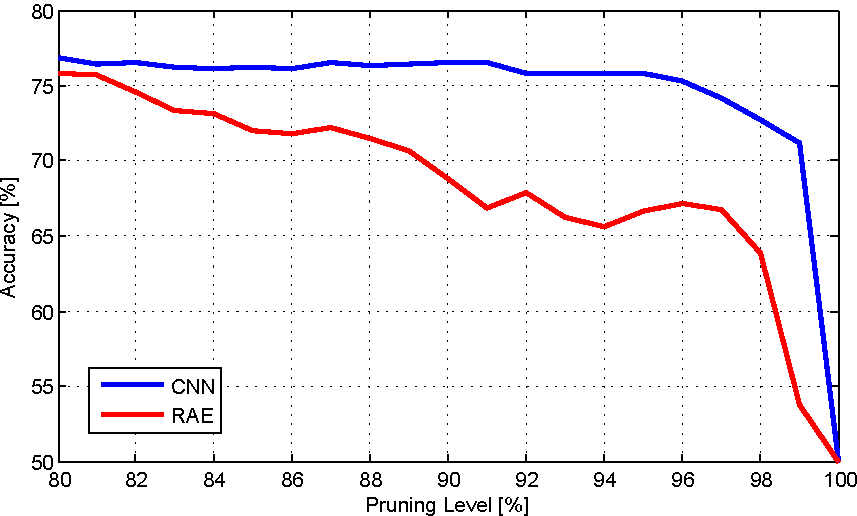
\includegraphics[width=0.55\textwidth]{Figures/pruning80-100-all_small.pdf}
    \caption{Binary sentiment polarity classification accuracy of Logistic Regression. Underlying sentence representations were extracted with pruned versions of CNN or RAE at different pruning levels.}
  \label{fig:pruning}
%\end{figure}
\end{wrapfigure}

Figure \ref{fig:pruning} shows the accuracy of the Logistic Regression classifier after training it on the pruned SRAE and CNN sentence representations with random word vector initialization. In both models, we could prune up to 81\% of the parameters without observing any major impact on the classification accuracy induced by the modified phrase representations (not shown in the figure). In case of the CNN, even if we removed up to 95\% of all model parameters, the representations seem to preserve enough information about the inputs to be classified correctly with 76\% accuracy.

Small weight values only have modest impact on the net input of neurons in the network. Accordingly, a neuron's output does not change much in its activation with respect to changes in the inputs that are received from low-weight connections. In a neural network there are typically many settings of weights that could potentially model the dataset quite well - especially for small datasets and lots of parameters, like in our case.\\
The drop in the CNN's accuracy is rather small for pruning levels below 95\%, when it starts decreasing rapidly. With max-pooling, one essentially samples a particular instance from the set of potential network architectures which have the same weights (the one where only the neuron with maximum activation is included in the computation graph). Since the input weights of neurons in a convolutional layer are shared, pruning small weights, in many cases, does not change the selection of a neuron after applying the max-operation. Thus, the CNN's particular architecture to which the model converged to after training, is mostly unaffected by many settings of pruned weights.

\section{Conclusion}
We presented a comparison of the Semi-Supervised Recursive Autoencoder and a Convolutional Neural Network and evaluated the capability of both networks to extract sentence representations. From our experiments we conclude that a very simple CNN architecture with only one convolution and pooling layer can be as effective as the SRAE for sentiment polarity classification of sentences. We showed that word embeddings trained with the Skip-Gram language model on a corpus of subjective text does not significantly improve classification performance on this sentiment analysis task. A pruning experiment revealed that in both neural phrase models up to 81\% of all parameters can be omitted without causing a major impact on the learned phrase representations. This might point towards more efficient training methods for neural networks.

%
% ---- Bibliography ----
%
\begin{thebibliography}{5}

\bibitem{socher2010learning}
Socher, R., Manning, C. D., Ng, A. Y.:
Learning continuous phrase representations and syntactic parsing with recursive neural networks.
In Proceedings of the NIPS-2010 Deep Learning and Unsupervised Feature Learning Workshop, 1--9, (2010)

\bibitem{socher:2011}
Socher, R., Pennington, J., Huang, E. H., Ng, A. Y., Manning, C. D.:
Semi-supervised recursive autoencoder for predicting sentiment distributions.
In Proceedings of the Conference on Empirical Methods in Natural Language Processing, 151--161, (2011)

\bibitem{socher:2013b}
Socher, R., Perelygin, A., Wu, J. Y., Chuang, J., Manning, C. D., Ng, A. Y., Potts, C.:
Recursive deep models for semantic compositionality over a sentiment treebank.
In Proceedings of the Conference on Empirical Methods in Natural Language Processing, p. 1642,(2013b)

\bibitem{collobertweston}
Collobert, R., Weston, J.:
A unified architecture for Natural Language Processing: Deep neural networks with multitask learning. 
In Proceedings of the 25th International Conference on Machine Learning, 160-–167, (2008)

\bibitem{santos}
dos Santos, C. N., Gatti, M.:
Deep convolutional neural networks for sentiment analysis of short texts.
In Proceedings of the 25th International Conference on Computational Linguistics (COLING), (2014)

\bibitem{pollack}
Pollack, J. B.: Recursive distributed representations. Artificial Intelligence, 46(1), 77--105, (1990)

\bibitem{bopang}
Pang, B., Lee, L.:
Seeing stars: Exploiting class relationships for sentiment categorization with respect to rating scales.
In Proceedings of the 43rd Annual Meeting on Association Computational Linguistics, 115--124, (2005)

\bibitem{mikolov}
Mikolov, T., Sutskever, I., Chen, K., Corrado, G. S., Dean, J.:
Distributed representations of words and phrases and their compositionality.
In Advances in Neural Information Processing Systems 26, 3111–-3119, (2013)

\bibitem{mikolov:efficient}
Mikolov, T., Chen, K., Corrado, G., Dean, J.:
Efficient estimation of word representations in vector space.
arXiv preprint arXiv:1301.3781, (2013)

\end{thebibliography}

\end{document}
